\documentclass[,a4paper,12pt,french]{article}

\usepackage[TD]{../../../Style}

\pagestyle{empty}

\geometry{paperwidth=12cm,paperheight=9cm,margin=5mm}

% Début du document
%%%%%%%%%%%%%%%%%%%
\begin{document}

\begin{center}
\begin{tikzpicture}
\tkzTabInit[lgt=1.4,espcl=1.7]{$x$/1, $f(x)$/1}{$-4$,$-2$,3,7}
\tkzTabLine{,+,z,-,z,+,}
\end{tikzpicture}

\begin{tikzpicture}
\begin{axis}[
styleglobal,
width=0.8*\linewidth,
xmin=-4.5, xmax= 7.5,
ymin=-2.5, ymax=3.5,
xtick distance=1,
ytick distance=1,
minor x tick num=1,
minor y tick num=1,
labelgros,
]
\addplot[styleplot,domain=(0:8),tension=0.7] plot coordinates {(-4,2) (-2,0) (0,-2) (3,0) (7,1)} node[pos=0.75,above left] {$\mathscr C_1$} \pointsextremites;
\addplot[styleplot,color=DarkRed,densely dashed,tension=0.2] plot coordinates{(-4,-1) (-2,0) (0,-1) (3,-2) (7,2)} node[pos=0.7,below right] {$\mathscr C_2$} \pointsextremites;
\end{axis}
\end{tikzpicture}
\end{center}

\end{document}
